\chapter{Задание \textnumero2}

\section{Условие}
Реализовать три загружаемых модуля ядра: md1, md2, md3.

\subsection{md1}
Модуль md1 демонстрирует возможность создания экспортируемых данных и функции. Данныи модуль ядра должен содержать:
\begin{itemize}
    \item экспортируемые строковые (char *) и численные (int) данные;
    \item экспортируемые функции возвращающие строковые и числовые значения;
\end{itemize}

\subsection{md2}
Модуль md2 демонстрирует использование данных и функции, экспортируемых первым модулем (md1). Данныи модуль должен при загрузке:
\begin{itemize}
    \item вызывать все экспортированные модулем md1 процедуры и вывести в системныи журнал возвращаемые ими значения с указанием имени вызваннои процедуры;
    \item вывести в системныи журнал все экспортированные модулем md1
данные.
\end{itemize}

\subsection{md3}
Модуль md3 демонстрирует сценарии некорректного завершения установки модуля, и возможность использования загружаемого модуля в качестве функции, выполняемои в пространстве ядре. Процедура инициализации этого загружаемого модуля должна возвращать ненулевое значение и выводить в системныи журнал данные и возвращаемые значения экспортированных модулем md1 процедур (аналогично md2). Данныи модуль включен в работу для проработки вопросов, связанных с отладкои модулей ядра.

\section{Реализация}
\begin{lstlisting}[caption={Makefile}]
ifneq ($(KERNELRELEASE),)
	obj-m := md1.o md2.o md3.o
else
	CURRENT = $(shell uname -r)
	KDIR = /lib/modules/$(CURRENT)/build
	PWD = $(shell pwd)

default:
	$(MAKE) -C $(KDIR) M=$(PWD) modules

clean:
	rm -rf .tmp_versions
	rm *.ko
	rm *.o
	rm *.mod.c
	rm *.symvers
	rm *.order
endif
\end{lstlisting}
\begin{lstlisting}[caption={md1.h}]
#ifndef OSLAB03_MD1_H_
#define OSLAB03_MD1_H_

extern int   md1_int_data;
extern char *md1_str_data;

extern char *md1_get_str(int n);
extern int   md1_factorial(int n);

#endif // OSLAB03_MD1_H_
\end{lstlisting}
\begin{lstlisting}[caption={md1.c}]
#include "md1.h"

#include <linux/init.h>
#include <linux/module.h>

MODULE_LICENSE("GPL");
MODULE_AUTHOR("Faris Nabiev");

static int  __init my_module_init(void);
static void __exit my_module_exit(void);

module_init(my_module_init);
module_exit(my_module_exit);

int   md1_int_data = 255;
char *md1_str_data = "First module str data";

static int __init my_module_init(void)
{
    printk(KERN_INFO "Module 1 task_02: init\n");

    return 0;
}

static void __exit my_module_exit(void)
{
    printk(KERN_INFO "Module 1 task_02: unloaded\n");
}

extern char *md1_get_str(int n)
{
    printk(KERN_INFO "Module 1 task_02: md1_get_str(%d) has called\n", n);

    switch (n)
    {
        case 1:
            return "First message";

        case 2:
            return "Second message";

        default:
            return "Default message";
    }
}

extern int md1_factorial(int n)
{
    int i;
    int res = 1;

    printk(KERN_INFO "Module 1 task_02: md1_factorial(%d) has called\n", n);

    if (n > 1)
        for (i = 2; i <= n; i++)
            res *= i;

    return res;
}

// Экспорт данных
EXPORT_SYMBOL(md1_str_data);
EXPORT_SYMBOL(md1_int_data);
// Экспорт функций
EXPORT_SYMBOL(md1_get_str);
EXPORT_SYMBOL(md1_factorial);
\end{lstlisting}
\begin{lstlisting}[caption={md2.c}]
#include "md1.h"

#include <linux/init.h>
#include <linux/module.h>

MODULE_LICENSE("GPL");
MODULE_AUTHOR("Faris Nabiev");

static int  __init my_module_init(void);
static void __exit my_module_exit(void);

module_init(my_module_init);
module_exit(my_module_exit);

static int __init my_module_init(void)
{
    printk(KERN_INFO "Module 2 task_02: init\n");

    printk(KERN_INFO "Module 2 task_02: md1_int_data      = %d\n",
           md1_int_data);
    printk(KERN_INFO "Module 2 task_02: md1_str_data      = %s\n",
           md1_str_data);
    printk(KERN_INFO "Module 2 task_02: md1_get_str(10)   = %s\n",
           md1_get_str(10));
    printk(KERN_INFO "Module 2 task_02: md1_get_str(1)    = %s\n",
           md1_get_str(1));
    printk(KERN_INFO "Module 2 task_02: md1_get_str(2)    = %s\n",
           md1_get_str(2));
    printk(KERN_INFO "Module 2 task_02: md1_factorial(10) = %d\n",
           md1_factorial(10));

    return 0;
}

static void __exit my_module_exit(void)
{
    printk(KERN_INFO "Module 2 task_02: unloaded\n");
}
\end{lstlisting}
\begin{lstlisting}[caption={md3.c}]
#include "md1.h"

#include <linux/init.h>
#include <linux/module.h>

MODULE_LICENSE("GPL");
MODULE_AUTHOR("Faris Nabiev");

static int __init my_module_init(void);

module_init(my_module_init);

static int __init my_module_init(void)
{
    printk(KERN_INFO "Module 3 task_02: init\n");

    printk(KERN_INFO "Module 3 task_02: md1_int_data      = %d\n",
           md1_int_data);
    printk(KERN_INFO "Module 3 task_02: md1_str_data      = %s\n",
           md1_str_data);
    printk(KERN_INFO "Module 3 task_02: md1_get_str(10)   = %s\n",
           md1_get_str(10));
    printk(KERN_INFO "Module 3 task_02: md1_get_str(1)    = %s\n",
           md1_get_str(1));
    printk(KERN_INFO "Module 3 task_02: md1_get_str(2)    = %s\n",
           md1_get_str(2));
    printk(KERN_INFO "Module 3 task_02: md1_factorial(10) = %d\n",
           md1_factorial(10));

    return -1;
}
\end{lstlisting}

\section{Результаты работы}
\begin{figure}[H]
    \centering
    \caption{Сборка модулей}
    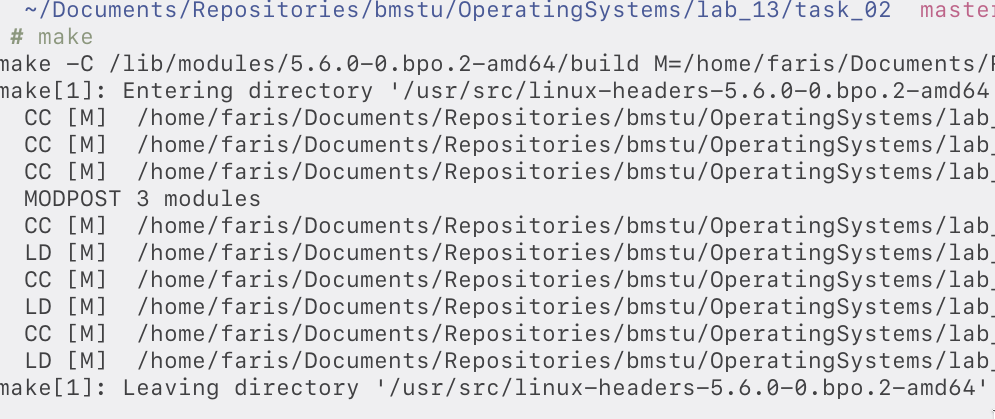
\includegraphics[scale=0.4]{images/scr_11.png}
\end{figure}
\begin{figure}[H]
    \centering
    \caption{Попытка загрузки модулей в неправильном порядке}
    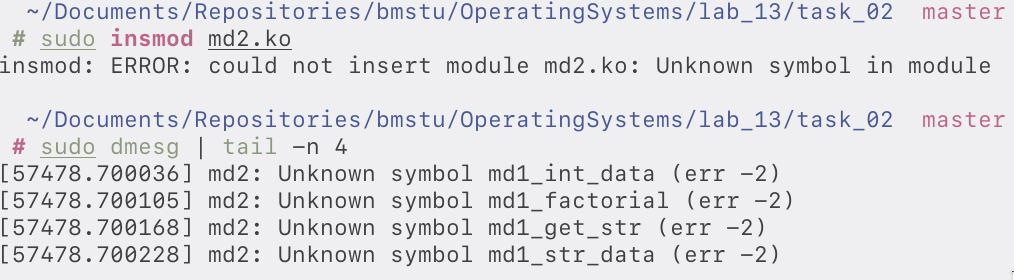
\includegraphics[scale=0.4]{images/scr_12.png}
\end{figure}

Причина возникшей ошибки заключается в том, что модуль md2 содержит ссылки на неизвестные ему имена. Значит, сначала нужно загрузичть модуль md1.

\begin{figure}[H]
    \centering
    \caption{Загрузка модулей в правильном порядке}
    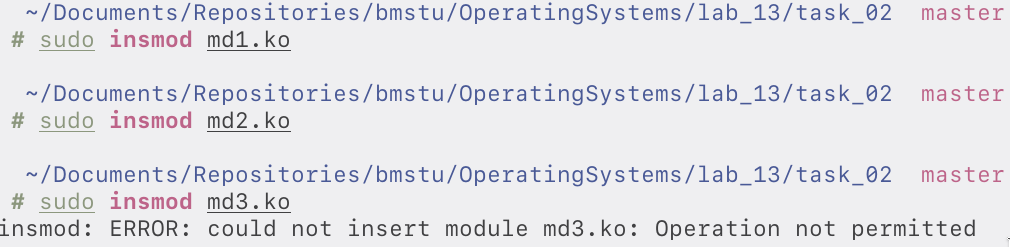
\includegraphics[scale=0.4]{images/scr_13.png}
\end{figure}

Модуль md3 не был загружен, потому что его функция инициализации возвращает -1.

\begin{figure}[H]
    \centering
    \caption{Проверка списка загруженных модулей}
    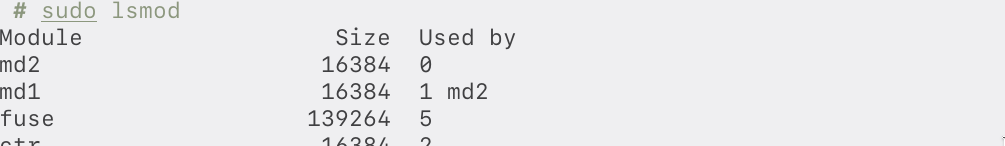
\includegraphics[scale=0.4]{images/scr_14.png}
\end{figure}
\begin{figure}[H]
    \centering
    \caption{Вывод буфера сообщений ядра}
    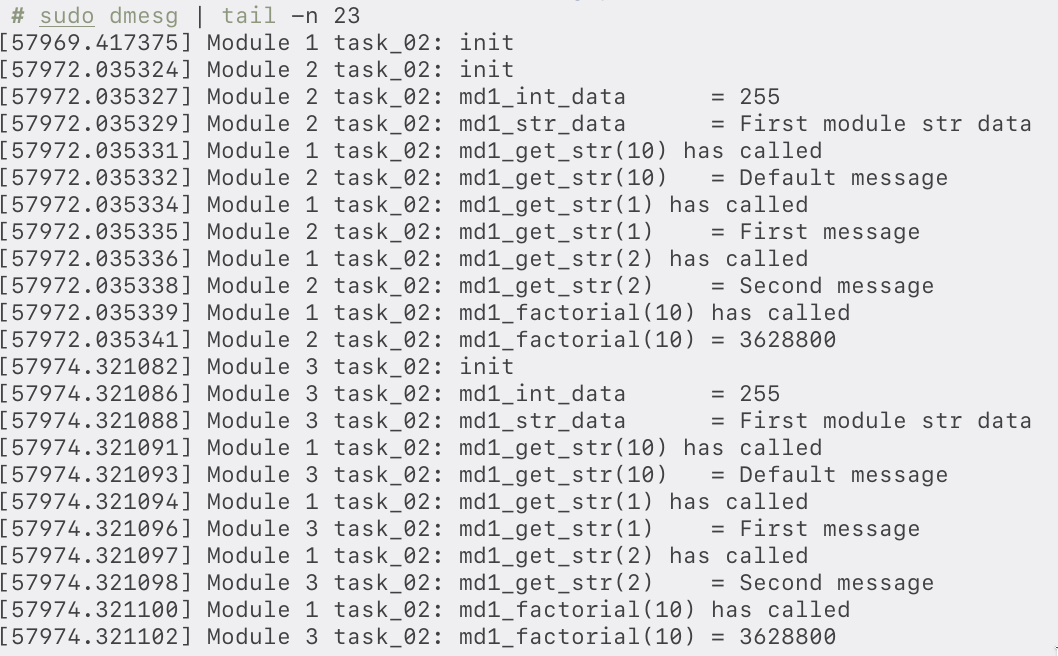
\includegraphics[scale=0.4]{images/scr_15.png}
\end{figure}
\begin{figure}[H]
    \centering
    \caption{Попытка выгрузки модулей в неправильном порядке}
    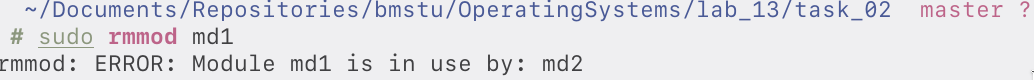
\includegraphics[scale=0.4]{images/scr_16.png}
\end{figure}

Попытка выгрузки модулей в неправильном порядке также вызывает ошибку.

\begin{figure}[H]
    \centering
    \caption{Выгрузка модулей в правильном порядке и вывод буфера сообщений ядра}
    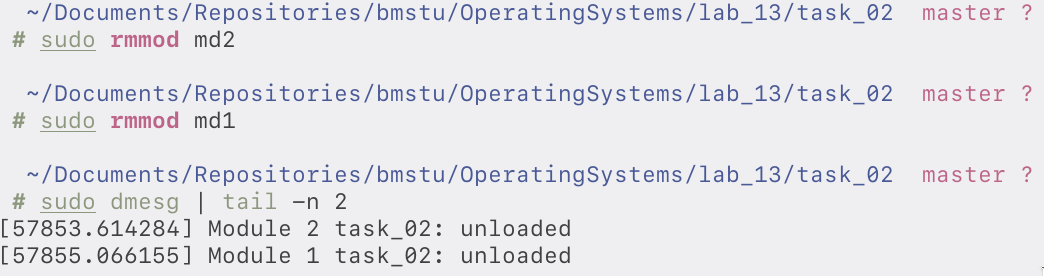
\includegraphics[scale=0.4]{images/scr_17.png}
\end{figure}
